%!TEX program = xelatex

\documentclass[a4paper, openany, oneside]{memoir}
\usepackage[no-math]{fontspec}
\usepackage{pgfplots}
\pgfplotsset{compat=newest}
\usepackage{commath}
\usepackage{mathtools}
\usepackage{amssymb}
\usepackage{amsthm}
\usepackage{booktabs}
\usepackage{mathtools}
\usepackage{xcolor}
\usepackage[separate-uncertainty=true, per-mode=symbol]{siunitx}
\usepackage[noabbrev, capitalize]{cleveref}
\usepackage{listings}
\usepackage[american inductor, european resistor]{circuitikz}
\usepackage{amsmath}
\usepackage{amsfonts}
\usepackage{ifxetex}
\usepackage[dutch,english]{babel}
\usepackage[backend=bibtexu,texencoding=utf8,bibencoding=utf8,style=ieee,sortlocale=en_GB,language=auto]{biblatex}
\usepackage[strict,autostyle]{csquotes}
\usepackage{parskip}
\usepackage{import}
\usepackage{standalone}
\usepackage{hyperref}
%\usepackage[toc,title,titletoc]{appendix}

\ifxetex{} % Fonts laden in het geval dat je met Xetex compiled
    \usepackage{fontspec}
    \defaultfontfeatures{Ligatures=TeX} % To support LaTeX quoting style
    \setromanfont{Palatino Linotype} % Tover ergens in Font mapje in root.
    \setmonofont{Source Code Pro}
\else % Terug val in standaard pdflatex tool chain. Geen ondersteuning voor OTT fonts
    \usepackage[T1]{fontenc}
    \usepackage[utf8]{inputenc}
\fi
\newcommand{\references}[1]{\begin{flushright}{#1}\end{flushright}}
\renewcommand{\vec}[1]{\boldsymbol{\mathbf{#1}}}
\newcommand{\uvec}[1]{\boldsymbol{\hat{\vec{#1}}}}
\newcommand{\mat}[1]{\boldsymbol{\mathbf{#1}}}
\newcommand{\fasor}[1]{\boldsymbol{\tilde{\vec{#1}}}}
\newcommand{\cmplx}[0]{\mathrm{j}}
\renewcommand{\Re}[0]{\operatorname{Re}}
\newcommand{\Cov}{\operatorname{Cov}}
\newcommand{\Var}{\operatorname{Var}}
\newcommand{\proj}{\operatorname{proj}}
\newcommand{\Perp}{\operatorname{perp}}
\newcommand{\col}{\operatorname{col}}
\newcommand{\rect}{\operatorname{rect}}
\newcommand{\sinc}{\operatorname{sinc}}
\newcommand{\IT}{\operatorname{IT}}
\newcommand{\F}{\mathcal{F}}

\newtheorem{definition}{Definition}
\newtheorem{theorem}{Theorem}


\DeclareSIUnit{\voltampere}{VA} %apparent power
\DeclareSIUnit{\pii}{\ensuremath{\pi}}

\hypersetup{%setup hyperlinks
    colorlinks,
    citecolor=black,
    filecolor=black,
    linkcolor=black,
    urlcolor=black
}

% Example boxes
\usepackage{fancybox}
\usepackage{framed}
\usepackage{adjustbox}
\newenvironment{simpages}%
{\AtBeginEnvironment{itemize}{\parskip=0pt\parsep=0pt\partopsep=0pt}
\def\FrameCommand{\fboxsep=.5\FrameSep\shadowbox}\MakeFramed{\FrameRestore}}%
{\endMakeFramed}

% Impulse train
\DeclareFontFamily{U}{wncy}{}
\DeclareFontShape{U}{wncy}{m}{n}{<->wncyr10}{}
\DeclareSymbolFont{mcy}{U}{wncy}{m}{n}
\DeclareMathSymbol{\Sha}{\mathord}{mcy}{"58}
\addbibresource{../../../../includes/bibliography.bib}

\begin{document}

\section{Collaborative sampling}

Collaborative sampling is very similar to circular sparse ruler, but differs in that it makes use of multiple devices. In this way, one device does not need to sample the information for all lags, because other devices might sample that information. This is illustrated in \cref{tkz:collaborative_ruler}, where $N=13$ and $M=4$ with two devices.

\begin{figure}[H]
\centering
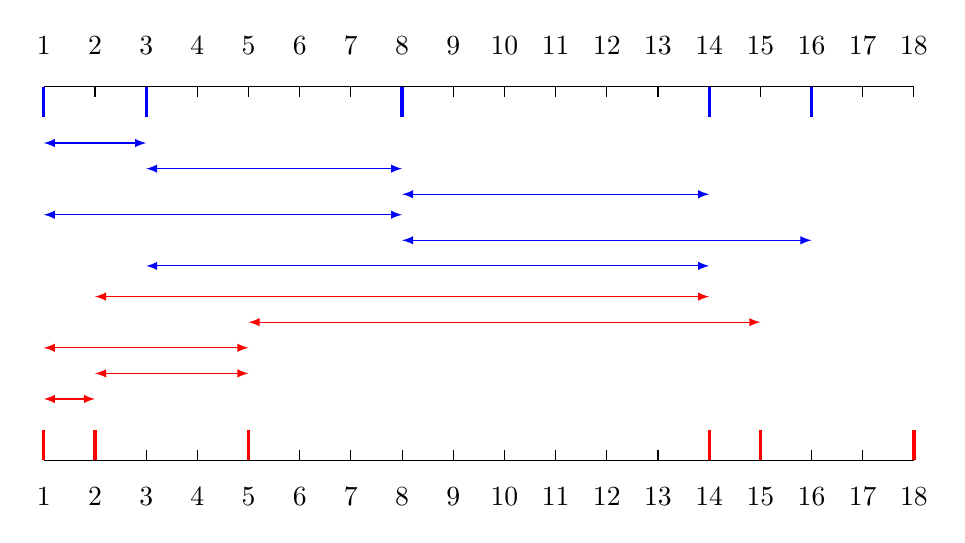
\begin{tikzpicture}[scale=1.3]

\draw (0,3.3) -- (8.5,3.3);
\draw [blue, very thick] (0,3) -- (0,3.3);
\draw (0.5,3.2) -- (0.5,3.3);
\draw [blue, very thick](1,3) -- (1,3.3);
\draw (1.5,3.2) -- (1.5,3.3);
\draw (2,3.2) -- (2,3.3);
\draw (2.5,3.2) -- (2.5,3.3);
\draw (3,3.2) -- (3,3.3);
\draw [blue, very thick](3.5,3) -- (3.5,3.3);
\draw (4,3.2) -- (4,3.3);
\draw (4.5,3.2) -- (4.5,3.3);
\draw (5,3.2) -- (5,3.3);
\draw (5.5,3.2) -- (5.5,3.3);
\draw (6,3.2) -- (6,3.3);
\draw [blue, very thick] (6.5,3) -- (6.5,3.3);
\draw (7,3.2) -- (7,3.3);
\draw [blue, very thick](7.5,3) -- (7.5,3.3);
\draw (8,3.2) -- (8,3.3);
\draw (8.5,3.2) -- (8.5,3.3);

\node at (0,3.7) {1};
\node at (0.5,3.7) {2};
\node at (1,3.7) {3};
\node at (1.5,3.7) {4};
\node at (2,3.7) {5};
\node at (2.5,3.7) {6};
\node at (3,3.7) {7};
\node at (3.5,3.7) {8};
\node at (4,3.7) {9};
\node at (4.5,3.7) {10};
\node at (5,3.7) {11};
\node at (5.5,3.7) {12};
\node at (6,3.7) {13};
\node at (6.5,3.7) {14};
\node at (7,3.7) {15};
\node at (7.5,3.7) {16};
\node at (8,3.7) {17};
\node at (8.5,3.7) {18};

\draw (0,-0.35) -- (8.5,-0.35);
\draw [red, very thick] (0,-0.35) -- (0,-0.05);
\draw [red, very thick](0.5,-0.35) -- (0.5,-0.05);
\draw (1,-0.35) -- (1,-0.25);
\draw (1.5,-0.35) -- (1.5,-0.25);
\draw [red, very thick](2,-0.35) -- (2,-0.05);
\draw (2.5,-0.35) -- (2.5,-0.25);
\draw (3,-0.35) -- (3,-0.25);
\draw  (3.5,-0.35) -- (3.5,-0.25);
\draw (4,-0.35) -- (4,-0.25);
\draw (4.5,-0.35) -- (4.5,-0.25);
\draw (5,-0.35) -- (5,-0.25);
\draw (5.5,-0.35) -- (5.5,-0.25);
\draw (6,-0.35) -- (6,-0.25);
\draw [red, very thick] (6.5,-0.35) -- (6.5,-0.05);
\draw [red, very thick](7,-0.35) -- (7,-0.05);
\draw (7.5,-0.35) -- (7.5,-0.25);
\draw (8,-0.35) -- (8,-0.25);
\draw [red, very thick](8.5,-0.35) -- (8.5,-0.05);

\node at (0,-0.7) {1};
\node at (0.5,-0.7) {2};
\node at (1,-0.7) {3};
\node at (1.5,-0.7) {4};
\node at (2,-0.7) {5};
\node at (2.5,-0.7) {6};
\node at (3,-0.7) {7};
\node at (3.5,-0.7) {8};
\node at (4,-0.7) {9};
\node at (4.5,-0.7) {10};
\node at (5,-0.7) {11};
\node at (5.5,-0.7) {12};
\node at (6,-0.7) {13};
\node at (6.5,-0.7) {14};
\node at (7,-0.7) {15};
\node at (7.5,-0.7) {16};
\node at (8,-0.7) {17};
\node at (8.5,-0.7) {18};

\draw [red, >=latex,<->] (0,0.25) -- (0.5,0.25);
\draw [blue, >=latex,<->](0,2.75) -- (1,2.75);
\draw [red, >=latex,<->](0.5,0.5) -- (2,0.5);
\draw [red, >=latex,<->](0,0.75) -- (2,0.75);
\draw [blue, >=latex,<->](1,2.5) -- (3.5,2.5);
\draw [blue, >=latex,<->](3.5,2.25) -- (6.5,2.25);
\draw [blue, >=latex,<->](0,2.05) -- (3.5,2.05);
\draw [blue, >=latex,<->](3.5,1.8) -- (7.5,1.8);
\draw [red, >=latex,<->](2,1) -- (7,1);
\draw [blue, >=latex,<->](1,1.55) -- (6.5,1.55);
\draw [red, >=latex,<->](0.5,1.25) -- (6.5,1.25);

\end{tikzpicture}
\caption{collaborative sampling solution for $N=13$ and $M=4$}\label{tkz:collaborative_ruler}
\end{figure}

The red arrows indicate the lags that are produced by device one, and the blue arrows indicate the lags that are produced by device two. Note that together they make all lags necessary.

The paper ref \todo{ref} investigates ways to come up with optimal set-ups for different amounts of devices. The solution presented in \cref{tkz:collaborative_ruler} is an optimal solution for two devices and three samplers: $S_1=\{1,2,4\}, S_2 = \{1,3,8\}$.

\subsection{combine collaborative sampler with reconstructor}\label{sub:ci-collab}
To describe how every sampler behaves to the different reconstructors, we can use the same technique as described in \cref{sub:ci-circ}. We need different devices to compute different parts of the desired autocorrelation $\vec{r}_x$. Therefore we have to tell the reconstructor to not try to reconstruct the whole autocorrelation, but only parts of it per device. The results of different devices are then combined. However, it is not trivial to tell the reconstructor to only calculate the parts of the autocorrelation it has information for. do this we need to take a look at

\begin{align} %\label{eq:ry-R-rx}
    \vec{r}_y = \mat{R} \vec{r}_x.
\end{align}
which is the result from \cref{eq:ry-R-rx} in ref \todo{ref}. This formula describes the relationship between $\vec{r}_y$ and $\vec{r}_x$. When we don't have all lags available, $\mat{R}$ is not full column rank, what in practice means that there are columns with only zeros. These columns correspond directly to the elements of $\vec{r}_x$ we have no information of. So what we now need to do is remove the columns with only zeros, and remove the corresponding elements out of $\vec{r}_x$. One can choose to either calculate beforehand which columns are zero, but one can also do that after calculating $\mat{R}$, and remove the columns that are zero. 

The only thing left to do is to combine the information on a combiner. This combiner takes the information of the different devices and puts their values accordingly in the autocorrelation vector $\vec{r}_x$. 


\end{document}
